\section{Our Implementation}
\label{sec:implementation}
\kento{In this section, we need to describe information, which should be
written in ``Developers' document''}

\begin{figure}
\centering
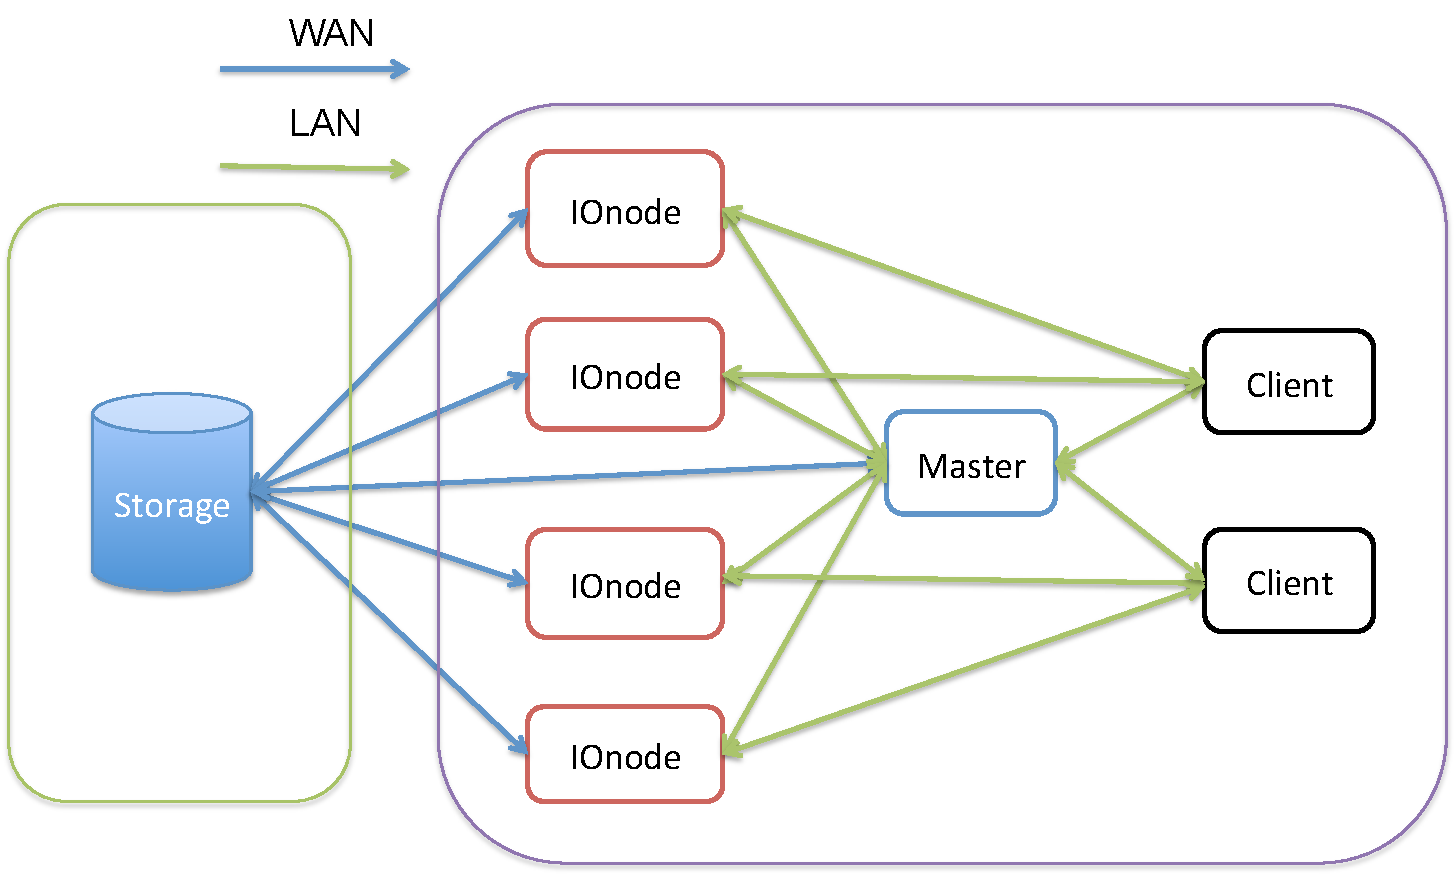
\includegraphics[width=8cm]{img/prototype_overview}
\caption{overview of prototype}
\label{implemetation:overview of prototype}
\end{figure}

In order to evaluate our architecture in a real environment and compare with current architecture,
we implemented a prototype.
In our architecture there are several global data such as total number of burst buffer nodes,
buffered file information need to be shared between all nodes.
And since in our proposal architecture, numbers of burst buffer nodes can be dynamically determined,
a global scheduler is needed to decide when and how nodes are added and removed, these decision
should be made based on global work load and local work load.
Also a scheduler is needed to handle the operation like re-balance of buffered data when nodes
addition, and data write back when nodes deletion.

For above reasons in this implementation, we adopted master-worker model, a master is designed to
store global information and interactive with client daemon, as well as serve as a scheduler.
The architecture of our prototype is described as Figure \ref{implemetation:overview of prototype}

In our architecture, there are three types of nodes:
\begin{itemize}
	\item A master node manages all burst buffer nodes information, maintains a set of buffered file
	meta data, handles operation like burst buffer node addition and deletion etc., and interact with
	clients.
	\item There are several burst buffer nodes response for actually storing data.
	\item A daemon runs on each client machine serving for communication with
	master and burst buffer nodes, in order to hide architecture detail from user.
\end{itemize}

The shared storage system are mounted on both master and burst buffer nodes, both of master and
burst buffer nodes have the same assess permission to the shared file system.

\subsection{File Chunk}
In our implementation, files are usually stored in more than one burst buffer node depends on the files'
size and numbers of burst buffer nodes available.
\xtq{detail chunk size}
Files are divided into dynamic determined-size \emph{chunks}, each burst buffer node store one chunk.
\kento{I think we should use another word instead of ``mutable''.
``configurable'' ?, ``dynamically changeable'', ``dynamically
optimized size ?'' ?}
Such one burst buffer node one chunk design simplified our data layout design, and operations in
burst buffer nodes addition and deletion.
\kento{I can not understand this. You mean if an application write X bytes
of data to N of burst buffer nodes, the system divide the data into N of chunks
with X/N bytes of size, OR totally mutable-size for each chunk ? Please send me
an email to answer as Q1} \kento{Q2: Given N of burst buffer nodes, can the
system divide the file into M (< N) ? Please send me an email to answer as Q2} For each chunk
we adopted a \emph{dirty flag}, in order to decide whether this chunk has been modified.
In write back phase, only the modified chunk needs to be written back to storage.
This dirty flag can reduce the write back data size and thus reduce the Internet congestion.

Applications usually generate various sizes of files, since in our architecture, memory is precious
resources, more memory means we can buffer more files, mutable size chunk design avoid the
disadvantage of memory waste in fixed-size chunk design, and enable us just to allocate requested size of memory.
\kento{I can not understand this because of Q1}
However such one burst buffer node one chunk design and mutable size has some disadvantages.
First master must maintain the chunk size of each file, this put a burden on master.
Second, for a large file the chunk size will become very large, cause a coarse-grained write back
control, and reduce the performance gained by dirty flag.
\kento{Q3: I can not understand why, because the chunk size is mutable. Please
send me an email to answer as Q3} Finally, since the chunk size is decided by
file size, and one burst buffer node store only one chunk, it is difficult to change buffered file size.

\subsection{Master Node}
In our master-worker node model, master node is the supervisor of the entire system,
master node is in charge of interactive with client, make file chunk placement, and handle file operations including file open, read and write.
Master node also manages the burst buffer nodes and schedule events like node registration at node
setup phase, addition and deletion.
In order to master node majorly maintains following two data structures:
\begin{itemize}
  \item burst buffer nodes information: including node IP address, total memory and
  available memory. 
  \item File meta data: including file path, file id, total file size, access control, chunk size,
  dirty flag and a map from chunks to burst buffer nodes.
\end{itemize}

Since only master has the global knowledge of file chunk placement, client must connect to master
to get these information.
\xtq{same file or different file}
However, in such master-worker model, master is easy to become a bottleneck of the whole system,
thus we have to minimize the master involvement in file operation, client asks master about the
file meta data, including the chunk placement information, then client uses these information and
connect to burst buffer nodes directly for sending or receiving data.

\subsection{Client daemon}

\begin{figure}[tb]
	\centering
	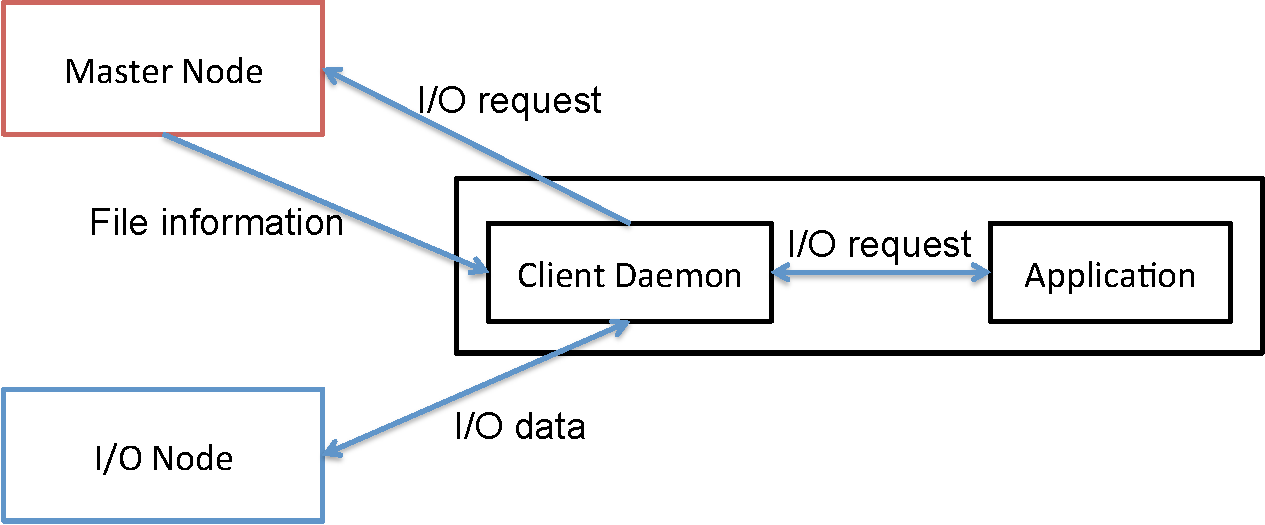
\includegraphics[width=8cm]{img/client_daemon}
	\caption{Client Daemon}
	\label{implementaion:client_daemon}
\end{figure}

In each compute node, there is a client daemon, which is a file system client used to buffer I/O
data, communicate with master nodes and burst buffer nodes, including send I/O request and send or
receive I/O data.
Figure.~\ref{implementaion:client_daemon} is an illustration of client daemon inside client nodes
and buffer queue in I/O burst nodes.
Applications changes data with client daemon by using mmap.
\kento{Q5: Is a client daemon really running on each client node ? Because you
say ``daemon'', I understand the daemon process is a different process to the
application's process. Is it true ? Please
send me an email to answer as Q5} Figure.~\ref{implementaion:client_daemon}
is an illustration of client daemon inside client nodes and buffer queue in burst buffer nodes.
Users don't know and should not know the information like IP address of master nodes,  client daemon
is used to hide these information from users.
By using client daemon, application doesn't need to change their code, just recompile with a
library.
As figure.~\ref{implementaion:client_daemon} shows, client daemon send open, close request to master
node, and cache the file information including file chunk size, a map to burst buffer nodes.
When applications send read and write request, daemon send the request to corresponding burst buffer nodes
according to the cached information from master node, and transfer data with burst buffer nodes, finally
send to applications.

%When a user application issue a write request, I/O data will be buffered in that node by client
%daemon, when user close the file, call flush function or I/O data size exceed I/O server buffer
%size, client daemon will try to transfer I/O data to buffer queue in I/O burst buffer, if buffer
%queue in not full, I/O data will be sent to I/O burst buffer via interconnection network and can be
% seen among computing nodes in the same system after that.
%However if buffer queue is full, client daemon will block user application and wait until buffer
%queue is ready to receive new I/O data, causing a low I/O throughput.

%Similarly when user issue a read request, there are two conditions: required file is buffered in
% buffer queue in I/O burst buffer, or file is stored only in storage in another system.
%In the first cases, file can be transferred to computing nodes from buffer queue directly, and can
% achieve a high throughput.
%If data is not in buffer queue, then a read operation described below will be executed, since data
% must be transferred from storage in another system, in this case, throughput will depend on Internet condition and it is hard to achieve a high throughput.

\subsection{File Operations}

\begin{figure}
\centering
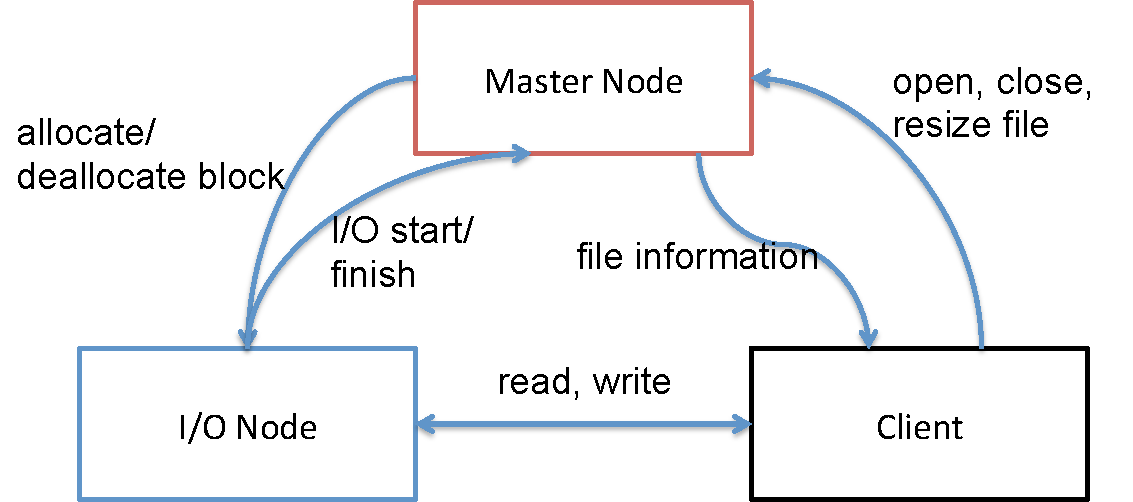
\includegraphics[width=8cm]{img/file_operation}
\caption{Details of File Operation}
\label{implementation:file operation}
\end{figure}

In this section we give more details about the file operation in our implementation, including
open, close, read and write.

When an application open a file, client daemon first send file path, access mode to master,
master return the file id,
for unbuffered file, master record the file information, and assign a file id, and then send the
file id to client daemon.

After file opened, applications can use file id to send read or write request.
In our prototype, since the master need to manage the block allocate and de-allocate operation, all
the read, write request should send to master.
When master receive the request, for file opened for reading
request for the first time, master get the file size from shared storage, and assign several burst
buffer nodes to this file according to file size and then send a map from chunks to burst buffer
node to client daemon, after that, master connects to corresponding burst buffer nodes, send allocate chunk request and
let burst buffer nodes read data from shared storage.
As for file opened in only writing since the file need to be create, master get file size from
client daemon and assign burst buffer nodes after that master send burst buffer nodes IP address as well as the map
information from chunks to burst buffer nodes to client daemon, then master connects to
corresponding burst buffer nodes, send allocate chunk request.

After receiving the map from chunks to burst buffer nodes, client daemon connect to each burst
buffer nodes in the map, and start I/O with these burst buffer nodes.

In order to monitor workload of each burst buffer nodes, and make load balanced, burst buffer nodes send a signal to
master at the start and the end of each data transfer.

\subsection{Limitation}

Since this is a prototype of our proposal system, there are several limitations.
First, in this prototype implementation, both master node and burst buffer nodes use one thread, it means
there is only one request can be responded at any time.
this design may cause master easily becoming a bottleneck when the number of client increase.
Also, since at any time one burst buffer node can transfer data with only one client, when the bandwidth of
burst buffer node larger than compute node, it will cause the burst buffer node under utilization.
However, there are some difficulties to change to a multiple threads version, for example, there
is a dependency between read from shared storage and send to compute nodes request, burst buffer nodes should
block the reading request from compute nodes until the read from shared storage finished also
synchronization is needed among read and write operations.

Second, one burst buffer node one data chunk design simplified master's design, but it also brings several
limitations. It is difficult to change the file size after buffered it, as well as it reduce the
benefit gain by using dirty flag.

Third, in the node addition and deletion, there is no load balance in our prototype.
Without load balance, after node added into the system, it needs a long time to achieve speed up.
Also in the node deletion, file write back and re-buffer are required.

In this paper, our aim is to validate effectiveness of burst buffers in
cloud.
Although we have these limitation in prototype, we can still show the effectiveness of burst
buffers.